\documentclass[11pt]{article}
\usepackage[margin=2.6cm]{geometry}
\usepackage{amsmath,amssymb}
\usepackage{xcolor}
\usepackage{tikz}
\usepackage{tikz-cd}
\usepackage{pgfplots}
\pgfplotsset{compat=1.18}
\usetikzlibrary{arrows.meta,positioning,calc,shapes.geometric}

% The paper's own colours and styles: the preview picks them up from this preamble.
\definecolor{amber}{HTML}{D79921}
\definecolor{ink}{HTML}{3C3836}
\tikzset{
  box/.style={draw=ink, rounded corners=2pt, minimum width=22mm, minimum height=8mm, font=\small},
  arrow/.style={-{Stealth[length=2.4mm]}, thick, draw=ink},
}

\title{TikZ in Scribe}
\author{A demo of Preview TikZ}
\date{}

\begin{document}
\maketitle

Put the cursor inside any picture below and press \textsf{Cmd+Opt+K} (Build $\to$ Preview TikZ).
The picture is drawn beside the source and redrawn as you type; moving the cursor into
another picture shows that one. On a blank line, the same command inserts a new figure to
start from.

\section{A diagram}
A pipeline drawn with the styles defined in the preamble. Try changing \texttt{amber} to
\texttt{red}, or adding a fourth box.

\begin{figure}[ht]
  \centering
  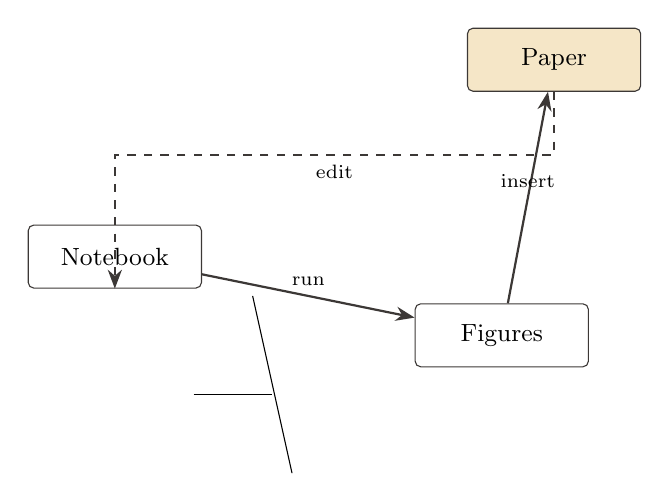
\begin{tikzpicture}[node distance=12mm]
    \node[box, yshift=1cm] (nb) {Notebook};
    \node[box, right=of nb, xshift=1.5cm, yshift=-1cm] (fig) {Figures};
    \node[box, right=of fig, fill=amber!25, yshift=3.5cm, xshift=-2.75cm] (paper) {Paper};
    
    \draw[arrow] (nb) -- node[above, font=\scriptsize] {run} (fig);
    \draw[arrow] (fig) -- node[above, font=\scriptsize] {insert} (paper);
    \draw[arrow, dashed] (paper.south) -- ++(0,-8mm) -| node[pos=.25, below, font=\scriptsize] {edit} (nb.south);
    \draw (1,-0.75) -- (2,-0.75);
    \draw (1.75,0.5) -- (2.25,-1.75);
  \end{tikzpicture}
  \caption{From notebook to paper.}
  \label{fig:pipeline}
\end{figure}

\section{A plot}
A pgfplots axis. Change the function or the domain and watch the curve move.

\begin{figure}[ht]
  \centering
  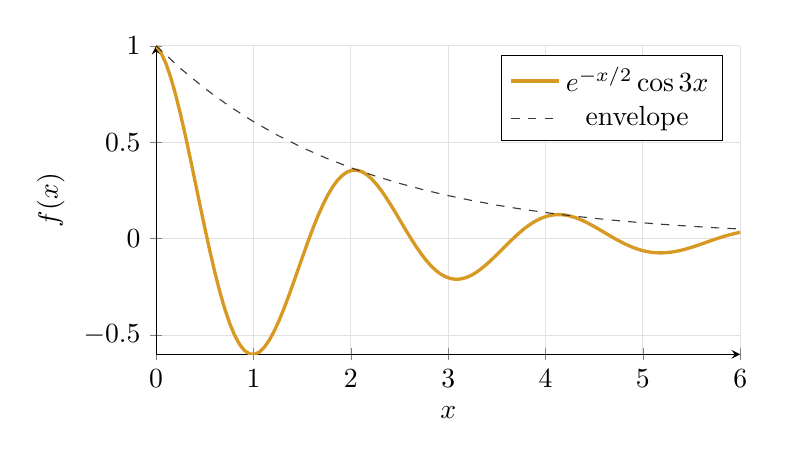
\begin{tikzpicture}
    \begin{axis}[width=9cm, height=5.5cm, xlabel={$x$}, ylabel={$f(x)$},
                 axis lines=left, grid=major, grid style={ink!15}, legend pos=north east]
      \addplot[amber, very thick, domain=0:6, samples=120] {exp(-x/2)*cos(deg(3*x))};
      \addplot[ink, dashed, domain=0:6] {exp(-x/2)};
      \legend{$e^{-x/2}\cos 3x$, envelope}
    \end{axis}
  \end{tikzpicture}
  \caption{A damped oscillation.}
  \label{fig:damped}
\end{figure}

\section{Geometry}
Coordinates, angles and a little arithmetic with \texttt{calc}.

\begin{figure}[ht]
  \centering
  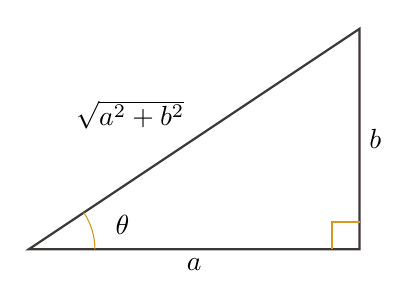
\begin{tikzpicture}[scale=1.4]
    \coordinate (O) at (0,0);
    \coordinate (A) at (3,0);
    \coordinate (B) at (3,2);
    \draw[thick, ink] (O) -- (A) -- (B) -- cycle;
    \draw[amber, thick] (A) ++(-.25,0) -- ++(0,.25) -- ++(.25,0);
    \draw[amber] (O) ++(.6,0) arc[start angle=0, end angle={atan(2/3)}, radius=.6];
    \node at ($(O)+(.85,.22)$) {$\theta$};
    \node[below] at ($(O)!.5!(A)$) {$a$};
    \node[right] at ($(A)!.5!(B)$) {$b$};
    \node[above left] at ($(O)!.5!(B)$) {$\sqrt{a^2+b^2}$};
  \end{tikzpicture}
  \caption{A right triangle.}
  \label{fig:triangle}
\end{figure}

\section{A commutative diagram}
\texttt{tikzcd} pictures preview the same way.

\[
\begin{tikzcd}
  A \arrow[r, "f"] \arrow[d, "g"'] & B \arrow[d, "h"] \\
  C \arrow[r, "k"'] \arrow[ur, dashed, "\exists!" description] & D
\end{tikzcd}
\]

\section{A network}
Loops with \texttt{\textbackslash foreach}: change the layer sizes to redraw the network.

\begin{figure}[ht]
  \centering
  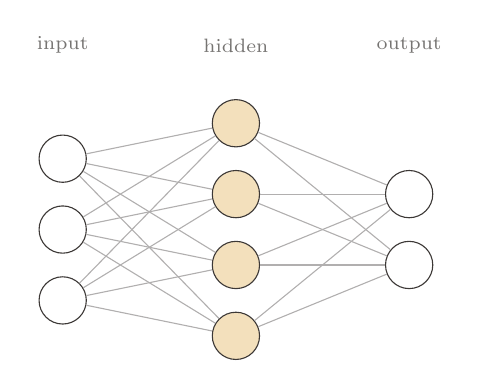
\begin{tikzpicture}[x=22mm, y=9mm, neuron/.style={circle, draw=ink, fill=white, minimum size=6mm},
                      hidden/.style={fill=amber!30}, input/.style={}, output/.style={}]
    \foreach \n/\layer [count=\l] in {3/input, 4/hidden, 2/output} {
      \foreach \i in {1,...,\n}
        \node[neuron, \layer] (\layer-\i) at (\l, {(\n+1)/2-\i}) {};
      \node[font=\scriptsize, ink!70] at (\l, 2.6) {\layer};
    }
    \foreach \i in {1,...,3} \foreach \j in {1,...,4} \draw[ink!40] (input-\i) -- (hidden-\j);
    \foreach \i in {1,...,4} \foreach \j in {1,...,2} \draw[ink!40] (hidden-\i) -- (output-\j);
  \end{tikzpicture}
  \caption{A small network.}
  \label{fig:network}
\end{figure}

\section{Scopes}
Points inside shifted, rotated and scaled scopes can be dragged too: hover over the picture to
see them, and drag one.

\begin{figure}[ht]
  \centering
  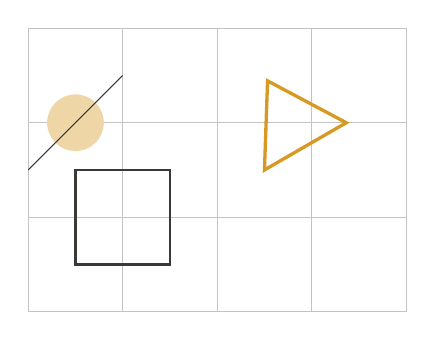
\begin{tikzpicture}[scale=1.2]
    \draw[ink!30] (0,0) grid (4,3);
    \draw[ink, thick] (0.5,0.5) rectangle (1.5,1.5);
    \begin{scope}[shift={(2.5,1.5)}, rotate=30]
      \draw[amber, very thick] (0,0) -- (1,0) -- (0.5,0.8) -- cycle;
    \end{scope}
    \begin{scope}[xshift=0.5cm, yshift=2cm, scale=0.5]
      \fill[amber!40] (0,0) circle (0.6);
      \draw[ink] (-1,-1) -- (1,1);
    \end{scope}
  \end{tikzpicture}
  \caption{Scopes move and turn what is inside them.}
  \label{fig:scopes}
\end{figure}

\section{Draw here}
A canvas to try the drawing tools on. Pick the arrow tool (A) and drag from one box to another:
the arrow is written as \texttt{(in) -{}- (out)}, so it follows the boxes when you move them.
Click a shape to select it and change its colour, width or dash in the style bar; double-click a
box to change its text.

\begin{figure}[ht]
  \centering
  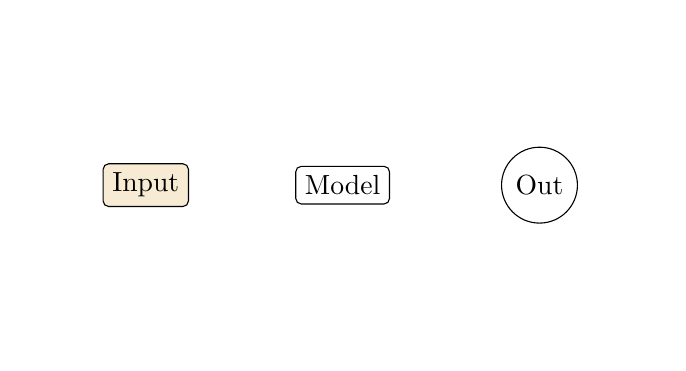
\begin{tikzpicture}
    \path[use as bounding box] (0,0) rectangle (8,4);
    \node[draw, rounded corners=2pt, fill=amber!20] (in) at (1.5,2) {Input};
    \node[draw, rounded corners=2pt] (model) at (4,2) {Model};
    \node[draw, circle] (out) at (6.5,2) {Out};
  \end{tikzpicture}
  \caption{Connect the boxes.}
  \label{fig:draw}
\end{figure}

\section{A picture in its own file}
\texttt{pictures/spiral.tikz} holds only the picture, and the paper inputs it. Open the file and
preview it: it still uses the paper's colours.

\begin{figure}[ht]
  \centering
  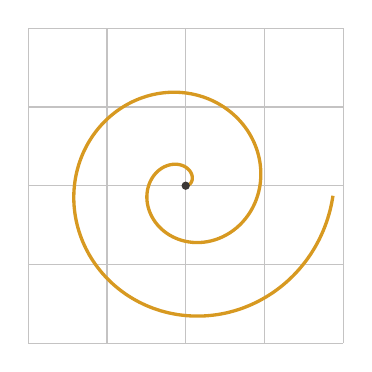
\begin{tikzpicture}
  \draw[ink!30] (-2,-2) grid (2,2);
  \draw[amber, very thick, domain=0:12.5, samples=200, smooth, variable=\t]
    plot ({0.15*\t*cos(\t r)}, {0.15*\t*sin(\t r)});
  \fill[ink] (0,0) circle (1.5pt);
\end{tikzpicture}

  \caption{An Archimedean spiral.}
  \label{fig:spiral}
\end{figure}

\section{Errors}
Uncomment the line below and the preview shows the error with a button that jumps to the
line in this file.

\begin{figure}[ht]
  \centering
  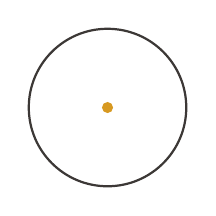
\begin{tikzpicture}
    \draw[ink, thick] (0,0) circle (1);
    \fill[amber] (0,0) circle (2pt);
    % \drwa (0,0) -- (1,1);  % a misspelt command
  \end{tikzpicture}
  \caption{Try breaking me.}
  \label{fig:broken}
\end{figure}

\end{document}
